
\subsection{Delayed Cause-and-Effect Tasks} \label{synth-benchmark:cause}



\looseness-1 To evaluate TGL methods' ability to learn delayed causal effects, we introduce the \emph{delayed cause-and-effect tasks}. In these tasks, we sample a sequence of graphs from a distribution (e.g., Erd\H{o}s-Rényi). A special node, called the memory node, is then added at each time step and connected to nodes involved in edges \(\lag\) time steps earlier. We formalize the task as follows:

\begin{definition}[Delayed Cause-and-Effect Task]
Let \(\lag \in \mathbb{N}\). The \emph{delayed cause-and-effect task} family \(\causeeffect{\lag}\) consists of dynamic graphs \(\mathcal{G} = G_1, G_2, \dots\) generated as follows: First, each graph \(G_t = (V, E_t)\) is sampled independently from a distribution \(D\) over static graphs, where \(V = \{v_1, \dots, v_N\}\) is the set of nodes, shared across time steps. For \(t > \lag\), the graph \(G_t\) is augmented by introducing a memory node \(v_{\mathcal M}\) and connecting it to the nodes involved in edges at time \(t - \lag\):
\[
V \leftarrow V \cup \{v_{\mathcal M}\}, \quad E_t \leftarrow E_t \cup \left\{ (v_{\mathcal M}, u), (v_{\mathcal M}, v) \mid (u,v) \in E_{t-\lag} \right\}  \text{ for } t > \lag.
\]
\end{definition}


 \begin{figure}[t]
    \centering
    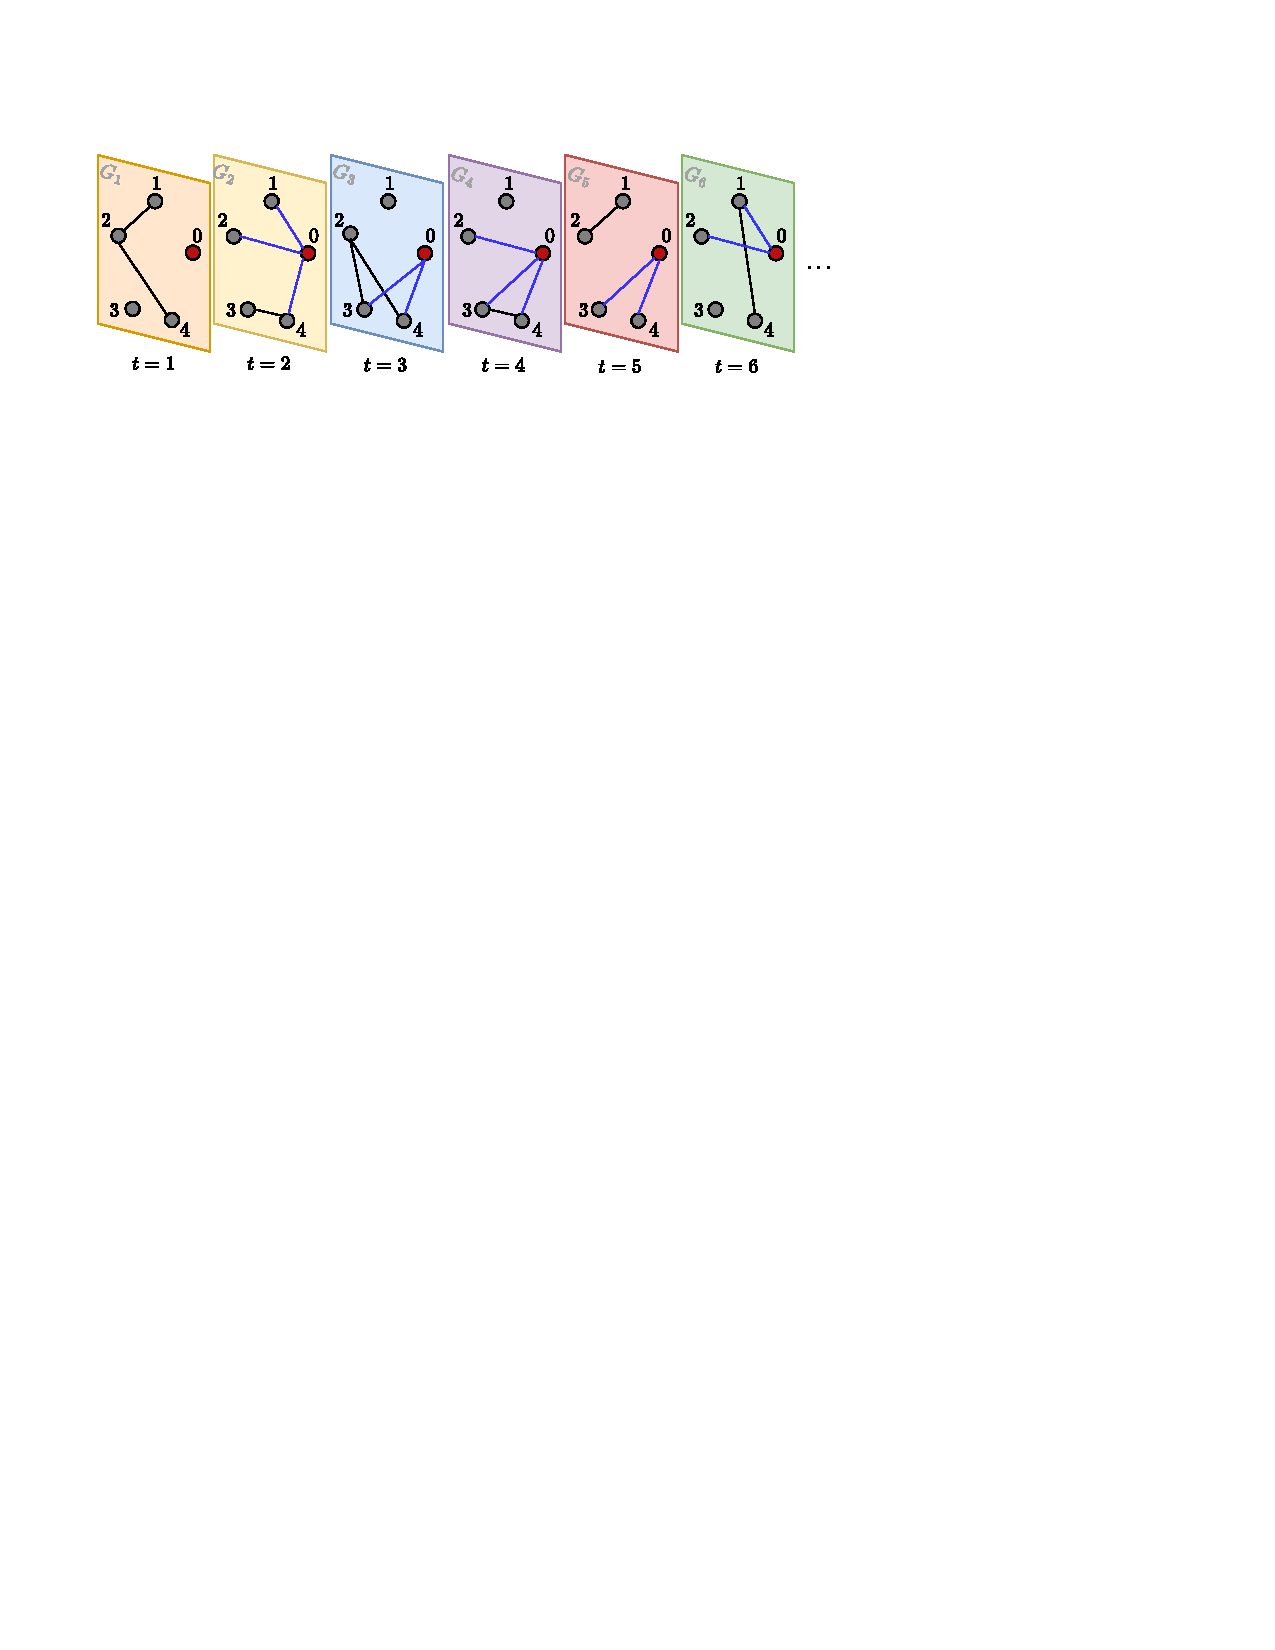
\includegraphics[width=0.8\linewidth, height=8em, keepaspectratio]{figs/memory_node/lag=1.pdf}
    \caption{Illustration of a delayed cause-and-effect dataset with lag $\lag=1$. \underline{Black edges} show the cause subgraph (nodes 1 to $N$). \underline{\textcolor{blue}{Blue edges}} show the effect subgraph, where the memory node (0) connects to previously active cause nodes (degree $\geq$ 1). }
    \label{fig:memnode}
\end{figure}

\looseness-1 Intuitively, the model needs to remember nodes that were connected to each other at $E_{t-\ell}$ to predict the edges of the memory node at time $E_t$. An example of this task is illustrated in Figure~\ref{fig:memnode}. As \(\lag\) increases, the task becomes more challenging in terms of the memory capacity required from the model. While the number of nodes and edges in the graphs \(G_t\) also affect the task's difficulty, we focus on varying \(\lag\). Since only the edges involving the memory node can be predicted~(the other ones being completely random), only the $F_1$ over possible edges involving the memory node are reported in our experiments.



\paragraph{Task objectives and implementation}
In the delayed cause-and-effect tasks \(\causeeffect{\lag}\), TGNNs must not only propagate information over time (i.e., track which nodes were connected at time step \(t-\lag\)), but also identify the causal relationship that determines the memory node's connectivity. This requires models to recognize causal patterns through time. The difficulty of the task is controlled by the hyperparameter \(\lag\): as \(\lag\) increases, the model needs to retain information for longer periods, making it harder to identify the cause-and-effect relationships. 
The graphs (except for the memory node) for this task are sampled from the ER model with 100 nodes and edge probability 0.01. 
%We used the Erdős–Rényi model~\cite{erdos1960evolution} with a connection probability of $p  = 0.002$ to sample the graphs with $100$ nodes. This low edge probability ensures sparsity, preventing memory nodes from connecting to most other nodes at each timestep. 
%We sample $4000 + \ell$ timesteps, ensuring the effect subgraph is present during the final $4000$ steps. \at{Task splits should be put into Appendix} The dynamic graph $\mathcal{G}$ is then split into 80/10/10\% for training, validation, and testing. \at{This can be shorter (see previous section)} To progressively increase the task’s temporal complexity and observe how model behaviors evolve, we varied the lag values across $\{1, 4, 16, 64, 256\}$, as further discussed in the following section.


\begin{wrapfigure}{l}{0.5\textwidth}
    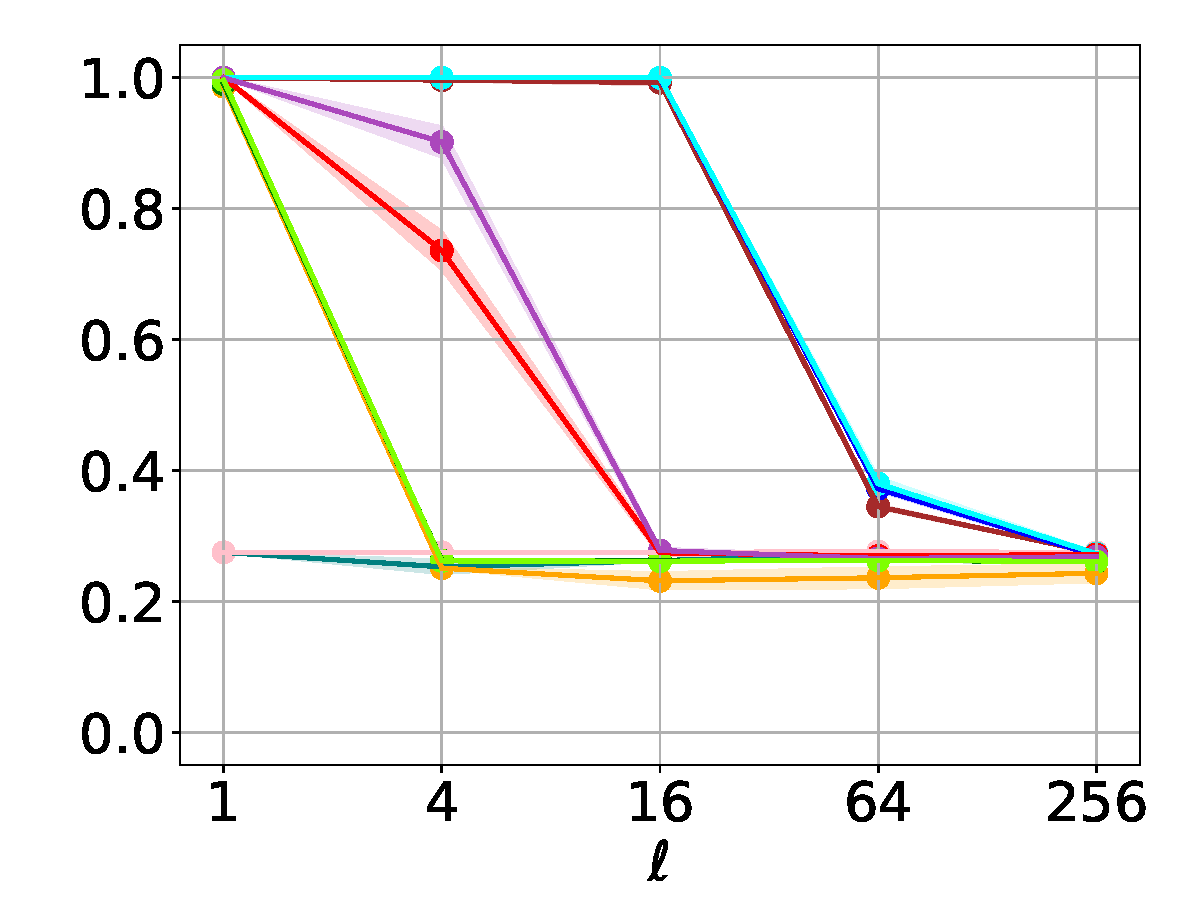
\includegraphics[width=0.7\linewidth]{figs/memory_node/(8, 6)/(l)Best_Test $F_1$.pdf}
    \raisebox{5mm}{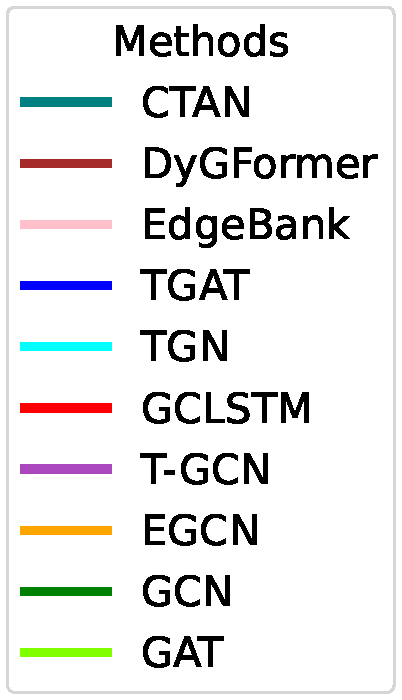
\includegraphics[width=0.2\linewidth]{figs/legends/CTDG DTDG all w edgebank wo persistence.pdf}}
        \caption{Methods' performance on cause-and-effect tasks $\causeeffect{\ell}$ across five temporal lags $\ell$.}
    \label{fig:plot_mem_node}
\end{wrapfigure}
\textbf{Results.}
Figure~\ref{fig:plot_mem_node} shows results on cause-and-effect tasks. At short lags (e.g., $\ell = 1$), most methods perform well, as there's almost no time element and we just need to extract information from the last input, making it an easy task where even static models can capture short-range dependencies. However, performance drops as lag increases, with both static and DTDG methods struggling to model longer temporal dependencies. GC-LSTM and T-GCN, in particular, show sharp declines at $\ell = 4$ and $\ell = 16$, reflecting the difficulty recurrent models face in retaining long-term information. In contrast, DyGFormer, TGAT, and TGN consistently outperform others, highlighting the strengths of attention and memory mechanisms in modeling dynamic temporal patterns. At large lags ($\ell = 64$ and $\ell = 256$), all methods approach the performance of EdgeBank, revealing a general challenge in capturing long-term causal links. Notably, CTAN performs unreliably even at small lags, suggesting limited effectiveness in this setting. Overall, the results underscore the critical role of attention and memory in temporal reasoning over dynamic graphs.

% Figure~\ref{fig:plot_mem_node} presents the results on cause-and-effect tasks. At small lags (e.g., $\ell = 1$), most methods perform well, suggesting that even static graph models can reliably capture short-range cause-and-effect relationships. As the lag increases, however, both static graph learning and DTDG approaches quickly lose effectiveness in modeling longer temporal dependencies. Notably, GC-LSTM and T-GCN experience a sharp performance drop at $\ell = 4$ and $\ell = 16$, highlighting the challenges recurrent architectures face in retaining temporal information over extended sequences. In contrast, DyGFormer, TGAT, and TGN consistently outperform their counterparts, demonstrating the advantage of attention mechanisms and memory modules in modeling dynamic temporal patterns. At larger lags~($\ell = 64$ and $\ell = 256$), performance deteriorates for all methods approaching $F_1$ value close to the EdgeBank, exposing a general limitation in capturing very long-term causal dependencies in dynamic graphs. Interestingly, CTAN exhibits unstable and unreliable performance even at the smallest lag value, underscoring its limited capacity for identifying causal structures within this setting. These results emphasize the importance of architectural choices, particularly the integration of attention and memory components, for effectively handling temporal reasoning tasks in dynamic graph learning. 



% \begin{figure}[H]
%     % (k, 1) CTDG
%     \centering
%     \begin{subfigure}[b]{0.6\textwidth}
%     \centering
%     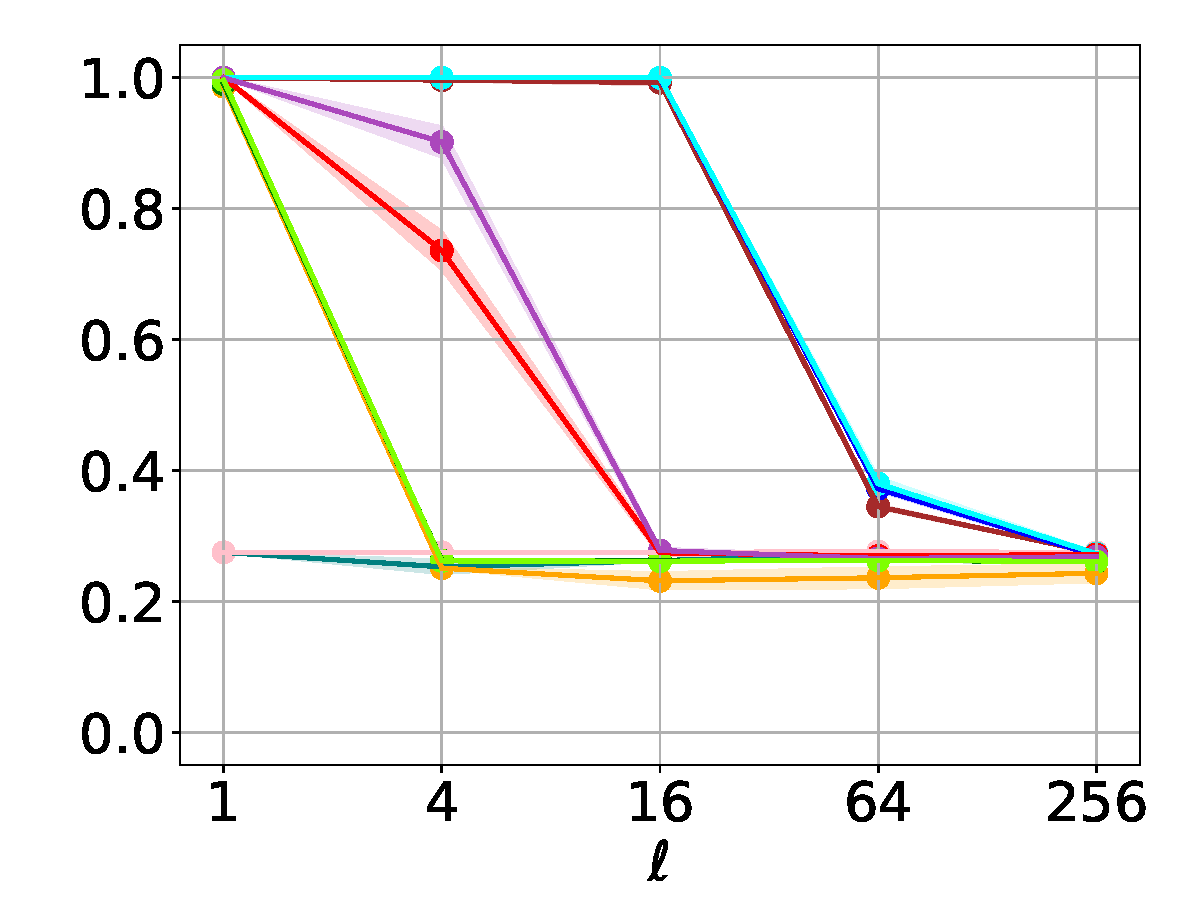
\includegraphics[width=\linewidth]{figs/memory_node/(8, 6)/(l)Best_Test $F_1$.pdf}
%     \end{subfigure}
%     \begin{subfigure}[b]{0.15\textwidth}
%         \centering
%         \raisebox{20mm}{
%     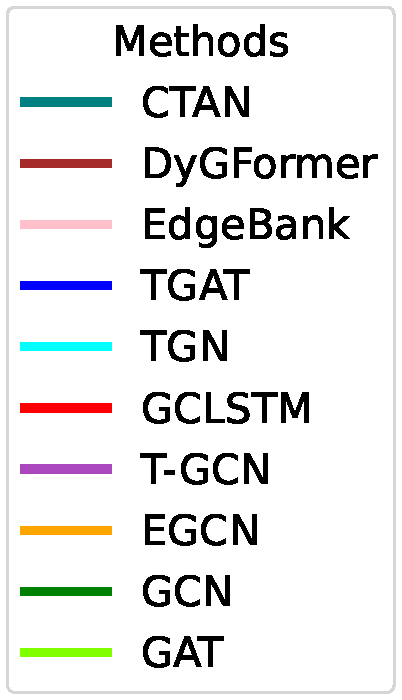
\includegraphics[width=\linewidth]{figs/legends/CTDG DTDG all w edgebank wo persistence.pdf}}
%         \end{subfigure}
%     \caption{Performance of methods on cause-and-effect tasks $\causeeffect{\ell}$ across five distinct temporal lags $\ell$.}
%     \label{fig:plot_mem_node}
% \end{figure}

% \begin{observation}[Cause and effect]
% DyGFormer, TGAT TGN are the best performing methods
% \end{observation}


% \subsubsection{Effect of number of neighbors}